\documentclass[11pt,a4paper,ngerman]{article}
\usepackage[bottom=2.5cm,top=2.5cm]{geometry} 
\usepackage{babel}
\usepackage[utf8]{inputenc} 
\usepackage[T1]{fontenc} 
\usepackage{ae} 
\usepackage{amssymb} 
\usepackage{amsmath}
\usepackage{amsthm} 
\usepackage{graphicx}
\usepackage{fancyhdr}
\usepackage{fancyref}
\usepackage{enumerate}
\usepackage{listings}
\usepackage{xcolor}
\usepackage{paralist}
\usepackage{tabularx}

\usepackage[pdftex, bookmarks=false, pdfstartview={FitH}, linkbordercolor=white]{hyperref}
\usepackage{fancyhdr}
\pagestyle{fancy}
\fancyhead[C]{Numerik I}
\fancyhead[L]{Übung 5}
\fancyhead[R]{SoSe 2013}
\fancyfoot{}
\fancyfoot[L]{}
\fancyfoot[C]{\thepage \hspace{1px} of \pageref{LastPage}}
\renewcommand{\footrulewidth}{0.5pt}
\renewcommand{\headrulewidth}{0.5pt}
\setlength{\parindent}{0pt} 
\setlength{\headheight}{0pt}

\date{Tutor : Christina Schulz}
\title{Übung 5}
\author{Max Wisniewski, Alexander Steen}


%%
%% Enviroments for proofs and lemmas
%%
\newtheorem{lemma}{\bfseries Claim}

\begin{document}

\lstset{language=Pascal, basicstyle=\ttfamily\fontsize{10pt}{10pt}\selectfont\upshape, commentstyle=\rmfamily\slshape, keywordstyle=\rmfamily\bfseries, breaklines=true, frame=single, xleftmargin=3mm, xrightmargin=3mm, tabsize=2, mathescape=true}

\renewcommand{\figurename}{Figure}

\maketitle
\thispagestyle{fancy}

%%%%%%%%%%%%%%%%%%%%%%%%%%%%%%
%% Aufgabe 1 %%%%%%%%%%%%%%%%
%%%%%%%%%%%%%%%%%%%%%%%%%%%%%%
\subsection*{Aufgabe 1}

Zeigen Sie, dass der Interpolationsoperator
\begin{equation*}
    \mathcal{C}[a,b] \ni f \mapsto \varphi (f) = p_n \in \mathcal{P}_n
\end{equation*}
eine Projektion ist und die Norm $\| \varphi \|_\infty = \Lambda_n$ hat, wobei
$$
    \Lambda_n = \underset{x \in [a,b]}{\max} \overset{n}{\underset{k=0}{\sum}} |L_k(x)|
$$
die Lebesque-Konstante ist und $L_k$ die Lagrange-Polyonme bezeichnet.\\

\textbf{Lösung:}\\

Seien $a \leq x_0 < ... < x_n \leq b$ die Stützstellen für den Interpolationsoperator.
Dann zeigen wir zunächst, dass für $f,g \in \mathcal{C}[a,b]$ und $\lambda \in \mathbb{R}$
\begin{equation*}
    \varphi(\lambda (f + g)) = \lambda (\varphi(f) + \varphi(g))
\end{equation*}
gilt.\\

\textbf{Beweis:}
Da der Interpolationsopertor nur über
\begin{equation}\label{numme:ueb5:intopdef}
    f(x_i) = \varphi(f)(x_i), \quad \forall 0 \leq i \leq n
\end{equation}
definiert ist, müssen wir auch nur jede der Stütztstellen untersuchen.\\

Sei $x_i$ eine der Stützstellen, beliebig aber fest.
\begin{equation}\begin{split}
    \varphi(\lambda (f + g))(x_i)
    &\stackrel{(\ref{numme:ueb5:intopdef})}{=} (\lambda (f + g))(x_i)\\
    &\stackrel{f,g\text{ stetig}}{=} \lambda (f(x_i) + g(x_i))\\
    &\stackrel{(\ref{numme:ueb5:intopdef})f,g}{=} \lambda (\varphi(f)(x_i) + \varphi(g)(x_i))\\
    &\stackrel{\varphi(f),\varphi(g)\text{ stetig}}{=} (\lambda (\varphi(f) + \varphi(g))) (x_i)
\end{split}\end{equation}
\mbox{}\hfill$\square$

Als nächstes zeigen wir, dass $\varphi^2 = \varphi$ ist.\\

\textbf{Beweis:}
Sei $f \in \mathcal{C}[a,b]$ beliebig aber fest.
Dann ist $p_n = \varphi(f) \in P_n$ ein Polynom vom Grad $n$.

Nun ist $q_n = \varphi(p_n) = \varphi^2(f) \in P_n$ ebenfalls ein Polynom vom Grad $n$,
bei dem nach Definition vom Interpolationsoperator gilt, dass
$\forall 0 \leq i \leq n \, : \, q_n(x_i) = p_n(x_i)$ gilt.

Nun gilt, dass zwei Polynome vom Grad $n$, die an $n+1$ Stellen den selben Wert haben die selben Polynome
sind. Also gilt $p_n = q_n$.\\
\mbox{}\hfill$\square$

Als nächstes zeigen wir, dass die Norm $\| \varphi \|_\infty = \Lambda_n$ ist.\\

\textbf{Beweis:}\\

Wir nehmen an, dass wir auf dem Zielraum $P_n$ wiederum die supremumsnorm verwenden wollen.

Es gilt zunächst, dass wenn wir ein Polynom haben, dass das Lagrangepolynom wieder das selbe beschreibt.
Das Lagrangepolynom $L(f)$ sieht wie folg aus.
\begin{equation}\begin{split}
    L(f)(x) &:= \overset{k}{\underset{j=0}{\sum}} y_i L_j(x)\\
        &\text{und}\\
    L(f)(x) = \varphi(L(f))(x) = \varphi(f)(x)
\end{split}\end{equation}

Zeigen wir zunächst, dass $\|\varphi\|_\infty \leq \Lambda_n$ ist.

\begin{equation*}\begin{split}
    \| \varphi \|_\infty  &= \underset{f \in \mathcal{C}[a,b]}{\sup} \| \varphi(f) \|_\infty \\
    &= \underset{f \in \mathcal{C}[a,b]}{\sup} \underset{x \in [a,b]}{\sup} |\varphi(f)(x)|\\
    &= \underset{f \in \mathcal{C}[a,b]}{\sup} \underset{x \in [a,b]}{\sup} |L(f)(x)|\\
    &= \underset{f \in \mathcal{C}[a,b]}{\sup} \underset{x \in [a,b]}{\sup} |\overset{k}{\underset{j=0}{\sum}} y_i L_j(x)|\\
    &\stackrel{\sup}{\leq} \underset{f \in \mathcal{C}[a,b]}{\sup} \underset{x \in [a,b]}{\sup} \overset{k}{\underset{j=0}{\sum}} |y_i L_j(x)|\\
    &\stackrel{\sup}{\leq} \underset{f \in \mathcal{C}[a,b]}{\sup} \underset{x \in [a,b]}{\max} \overset{k}{\underset{j=0}{\sum}} |L_j(x)|\\
    &= \underset{f \in \mathcal{C}[a,b]}{\sup} \Lambda_n\\
    &= \Lambda_n
\end{split}\end{equation*}

Und nun zeigen wir, dass $\Lambda_n \leq \|\varphi \|_\infty$ ist.

\begin{equation*}\begin{split}
    \Lambda_n &= \underset{x \in [a,b]}{\max} \overset{n}{\underset{k=0}{\sum}} |L_j(x)|\\
        &\leq \underset{x \in [a,b]}{\sup} \overset{n}{\underset{k=0}{\sum}} |L_j(x)|\\
        &\overset{\exists f\,:\,|y_i|\geq 1}{\leq} \underset{f \in \mathcal{C}[a,b]}{\sup} \underset{x \in [a,b]}{\sup} \overset{n}{\underset{k=0}{\sum}} |y_i||L_i(x)|\\
        &\leq \underset{f \in \mathcal{C}[a,b]}{\sup} \underset{x \in [a,b]}{\sup} \overset{n}{\underset{k=0}{\sum}} |y_i L_i(x)|\\
        &= \underset{f \in \mathcal{C}[a,b]}{\sup} \underset{x \in [a,b]}{\sup} \varphi(f)(x)\\
        &\stackrel{\text{Def.}}{=} \| \varphi \|_\infty
\end{split}\end{equation*}
\mbox{}\hfill$\square$

\subsection*{Aufgabe 2}

Betrachte die Funktionsklasse
\begin{equation*}
    \mathcal{F} = \{f \in C^{n+1}[-1,1] \, | \, \|f^{(n+1)}\|_\infty \leq (n+1)! \}.
\end{equation*}
Für $f \in \mathcal{F}$ bezeichne $p_n(f)$ das Interpolationspolynom $n$-ten Grades zu den Knoten
$K = \{t_0, ..., t_n \} \subset [-1,1]$.

\subsubsection*{(a)}

Zeigen Sie
\begin{equation*}
    \varepsilon_n(K) = \underset{f \in \mathcal{F}}{\sup} |f - p_n(f)| = \| \omega_{n+1} \|_\infty, \omega_{n+1}(t) = (t-t_0)...(t-t_n).
\end{equation*}

\textbf{Lösung:}\\
First we show that
\begin{equation*}\begin{split}
    \varepsilon_n(K)
    &= \underset{f \in \mathcal{F}}{\sup} \| f - p_n(f) \|_\infty\\
    &= \underset{f \in \mathcal{F}}{\sup}
        \underset{x \in [-1,1]}{\sup} | f (x) - p_n(f)(x) |\\
    &\stackrel{\text{Taylor}}{=} \underset{f \in \mathcal{F}}{\sup}
        \underset{x \in [-1,1]}{\sup} | T_n(x) + R_n(x) - p_n(T_n(x) + R_n(x)) |\\
    &\stackrel{\text{linear}}{=}\underset{f \in \mathcal{F}}{\sup} \underset{x \in [-1,1]}{\sup} | T_n(x) - p_n(T_n(x)) + R_n(x) - p_n(R_n(x)) |\\
    &\stackrel{T_n(x)=p_n(R_n(x))}{=} \underset{f \in \mathcal{F}}{\sup}\underset{x \in [-1,1]}{\sup} | R_n(x) - p_n(R_n(x)) | \\
    &= \underset{x \in [-1,1]}{\sup} \underset{f \in \mathcal{F}}{\sup}| \frac{f^{(n+1)}(\xi)}{(n+1)!} (x-a)^{n+1} - p_n(\frac{f^{(n+1)}(\xi)}{(n+1)!} (x-a)^{n+1}) |\\
    &\stackrel{f \in \mathcal{F}}{=} \underset{x \in [-1,1]}{\sup} | (x-a)^{n+1} - p_n((x-a)^{n+1}) |\\
    &\stackrel{\text{Lagrange Poylnom}}{=}
        \underset{x \in [-1,1]}{\sup}
    \left| (x-a)^{n+1} - \overset{n}{\underset{k=0}{\sum}} y_k L_k(x) \right|\\     
    &= \underset{x \in [-1,1]}{\sup}
     \left| (x-a)^{n+1} - 
    \overset{n}{\underset{k=0}{\sum}} y_k \underset{m \not= k}{\prod}
    \frac{x - t_m}{t_k - t_m} \right|\\
    &\stackrel{a = t_0}{=} \underset{x \in [-1,1]}{\sup}
        \left| (x-t_0)^{n+1} - \overset{n}{\underset{k=0}{\sum}} (t_k-t_0)^{n+1}
        \underset{m \not= k}{\prod} \frac{x - t_m}{t_k - t_m} \right| \\
    &= \underset{x \in [-1,1]}{\sup}
        \left| (x-t_0)^{n+1}-\overset{n}{\underset{k=1}{\sum}} (t_k - t_0)^{n+1}
        \underset{m \not= k}{\prod} \frac{x-t_m}{t_k - t_m} - (t_0-t_0)^{n+1}
        \underset{m \not= 0}{\prod} \frac{x - t_m}{t_0 - t_m} \right| \\
    &= \underset{x \in [-1,1]}{\sup}
        \left|  (x-t_0)^{n+1} - \underset{k=0}{\overset{n}{\prod}}(x-t_i)
        \overset{n}{\underset{k=1}{\sum}} 
        \frac{(t_k-t_0)^{n+1}}{(x-t_k)(x-t_0)}
        \underset{m \not= k}{\prod} \frac{1}{t_k - t_m}\right|\\
    &= \underset{x \in [-1,1]}{\sup}
        \left| \underset{k=0}{\overset{n}{\prod}} (x-t_i)
        \left( \underset{k=1}{\overset{n}{\prod}} \frac{x-t_0}{x-t_k}
        - \underset{k=1}{\overset{n}{\sum}}
        \frac{(t_k - t_0)^{n+1}}{(x-t_k)(x-t_0)}
        \underset{m\not= k}{\prod} \frac{1}{t_k - t_m} \right)\right|\\
    &\stackrel{(*)}{=} \underset{x \in [-1,1]}{\sup} \left| \underset{k=0}{
            \overset{n}{\prod}} x-t_i \right|\\
    &= \| w_{n+1}(x) \|_\infty
\end{split}\end{equation*}

Wir haben den Faden verloren und hoffen, dass bei $(*)$ der hintere
Teil $1$ sein sollte. Wir können gefahrlos durch unsere Definitionbereiche
teilen, da in $x \in K$ das Interpolationspolynom genau der ursprünglichen
Funktion entspricht. Daher wird dort auf jedenfall nicht das supremum
angenommen und wir können die übrigen stellen betrachten.

\subsubsection*{(b)}

Zeigen Sie $\varepsilon_n(K) \geq 2^{-n}$ und dass Gleicheit genau dann gilt, wenn $K$ die Menge
der Tschebyscheff-Knoten ist.\\

\textbf{Lösung:}\\

Wir wissen nun, dass
$\varepsilon_n(K) = \underset{x \in [-1,1]}{\sup} (x-t_0)\cdot ... \cdot(x - t_n)$
  
gilt. Nehmen wir an, es gibt ein Gitter, so dass
$\varepsilon_n(K) < 2^{-n}$. Dann gilt insbesondere, dass
$\omega_{n+1} (x) < 2^{-n}$ für alle $x \in [-1,1]$.

Nehmen wir $x=1$ als Punkt, so muss jeder Gitterpunkt
größer sein als
$1-2^{-n}$ sonst da sonst die Multiplikation zu groß wäre.\\
Nun gilt aber für $n\geq0$, dass für $k \in K$ $k > 0$ gelten müsste.
Damit wäre aber für $x = -1$ jede Differenz $x-k > 2^{-n}$ und folglich
ist $\omega_{n+1}(x) > 2^{-n}$.\\

Nun gilt zu zeigen, dass für Tschebyscheff-Knoten die Gleichheit erfüllt ist.\\

tbd

\subsection*{Aufgabe 3}


\subsubsection*{a)}
\begin{lstlisting}[language=matlab,numbers=left]
function v = AitkenNeville(x, fx, z)
% x Stuetzstellen
% fx Funktionswerte der Stuetzstellen
% z Auswertungsstelle

% n ist die Anzahl der Stuetzstellen
n = size(x,2);

% Initialwerte fuer alle p_11
for i = 1:n,
    p(i,i) = fx(i);
end;

% Nach dem Schema von Aitken
% Berechnung der restlichen Terme
for i = 1:n,
    for j = 1:n-i,
      p(j,j+i) = 1/(x(j+i)-x(j)) * ((z-x(j))*p(j+1,j+i) - (z-x(j+i))*p(j,j+i-1));
    end;
end;

% Rueckgabe ist p0n(x)
v = p(1,n);
\end{lstlisting}
\subsubsection*{b)}
\begin{lstlisting}[language=matlab,numbers=left]
function [] = InterpolationAD(f,I,n)
%% Grenzen des Intervalls
a = I(1);
b = I(2);
%% Genaugkeit des Plots
genauigkeit = 0.1;
dist = min(genauigkeit, (b-a)/n);

%% Erstelle Gitter:
%% Aequidistanter Gitter a = x0 < x1 < ... < xn = b
%% mit Distanz (b-a)/n
stuetzSt = [a:(b-a)/n:b];
%% Funktionswerte an den Stuetzstellen
fstuetzSt  = f(stuetzSt);

%% Erstelle Funktionswerte an allen Stellen
%% der gewaehlten Genauigkeit
%% unter Nutzung von Aitken-Neville
x  = [a:dist:b];
fx = zeros(1,length(x));
for i = 1:length(x)
  fx(i) = AitkenNeville(stuetzSt,fstuetzSt,x(i));
end;

%% Plot
plot(x,fx);
title('Interpolation durch Polynom n-ten Grades');
xlabel('x');
ylabel('p(x)');
\end{lstlisting}
\subsubsection*{c)}
\begin{lstlisting}[language=matlab,numbers=left]
function [] = InterpolationAD(f,I,n)
%% Grenzen des Intervalls
a = I(1);
b = I(2);
%% Genaugkeit des Plots
genauigkeit = 0.1;
dist = min(genauigkeit, (b-a)/n);

%% Erstelle Gitter:
%% Tschebyscheff-Gitter mit 
stuetzSt = zeros(1,n+1);
for i = 0:n
  stuetzSt(i+1) = a + ((b-a)/2) *(cos((2*i+1)/(2*(n+1)) * pi) + 1);
end;
%% Funktionswerte an den Stuetzstellen
fstuetzSt  = f(stuetzSt);

%% Erstelle Funktionswerte an allen Stellen
%% der gewaehlten Genauigkeit
%% unter Nutzung von Aitken-Neville
x  = [a:dist:b];
fx = zeros(1,length(x));
for i = 1:length(x)
  fx(i) = AitkenNeville(stuetzSt,fstuetzSt,x(i));
end;

%% Plot
plot(x,fx);
title('Interpolation durch Polynom n-ten Grades');
xlabel('x');
ylabel('p(x)');
\end{lstlisting}

\newpage
\subsubsection*{d)}
Als Funktionen zum Test wählen wir $x \mapsto \sin(x)$ und $x \mapsto e^x$, jeweils auf dem Intervall $[0,5]$.
Die Ergebnisse sind für Grad $n = 1,2,4$ folgende:  \\

\textbf{InterpolationAD}:\\
\begin{tabular}{l|ccc}
 & $n = 1$ & $n = 2$ & $n = 4$ \\
\hline
$\sin(x)$ & & & \\
& 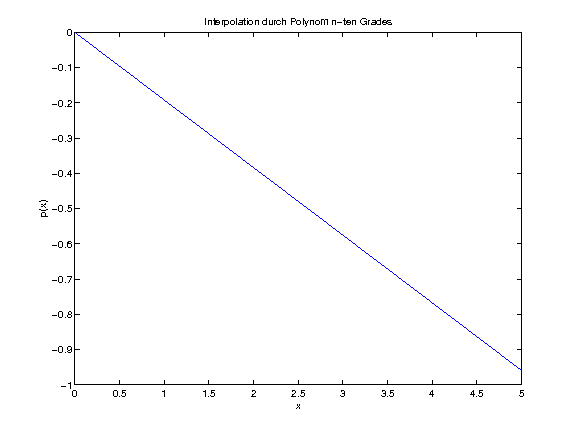
\includegraphics[width=0.3\textwidth]{plot1_1.png} & 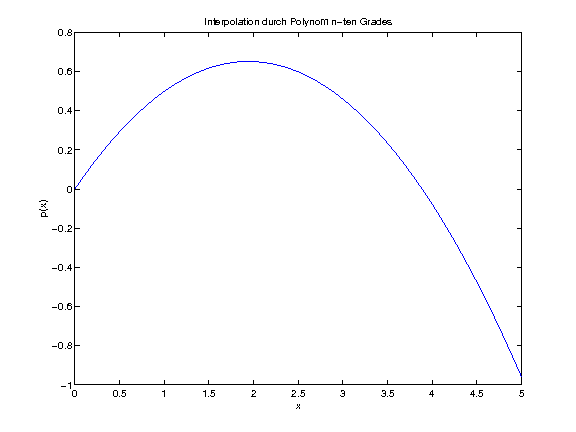
\includegraphics[width=0.3\textwidth]{plot1_2.png} & 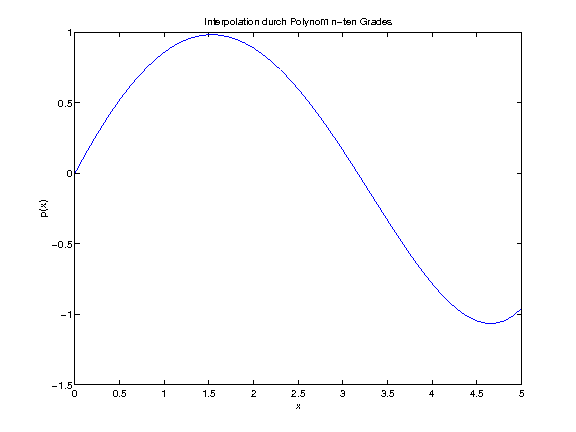
\includegraphics[width=0.3\textwidth]{plot1_4.png} \\
$e^x$ & & & \\
 & 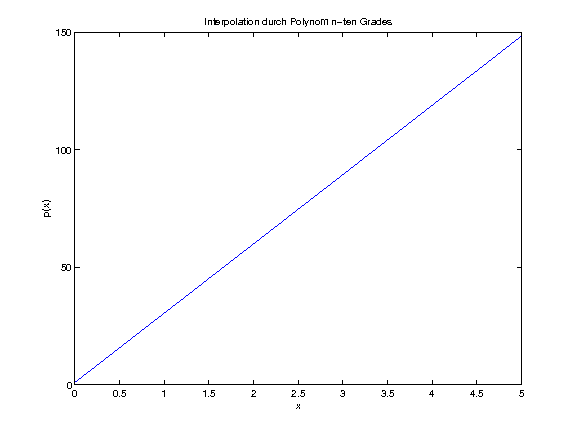
\includegraphics[width=0.3\textwidth]{plot2_1.png} & 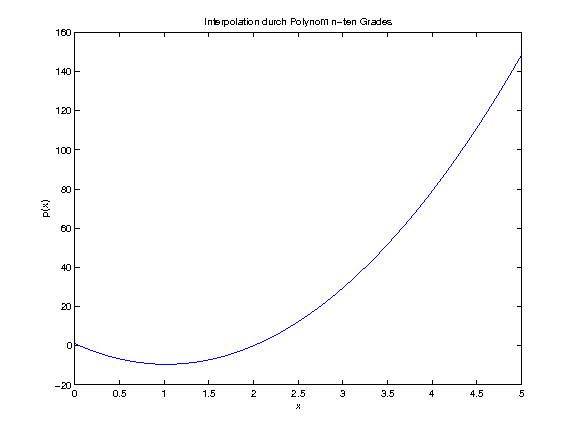
\includegraphics[width=0.3\textwidth]{plot2_2.png} & 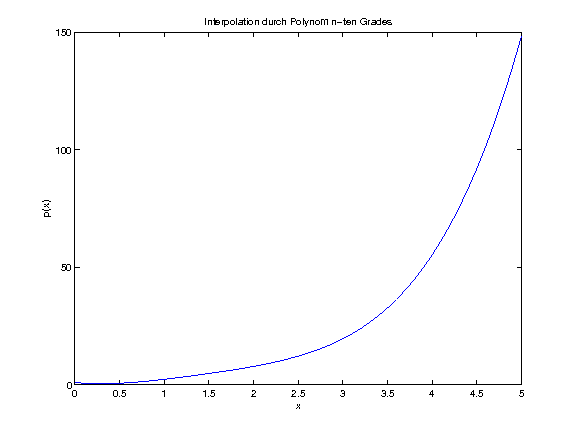
\includegraphics[width=0.3\textwidth]{plot2_4.png} \\
\end{tabular}

\textbf{InterpolationTscheby}:\\
\begin{tabular}{l|ccc}
 & $n = 1$ & $n = 2$ & $n = 4$ \\
\hline
$\sin(x)$ & & & \\
 & 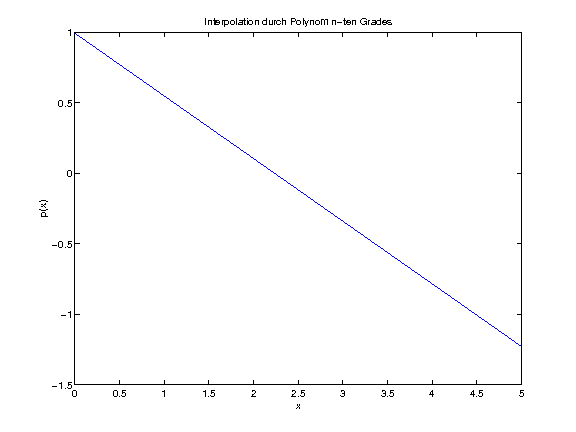
\includegraphics[width=0.3\textwidth]{plot4_1.png} & 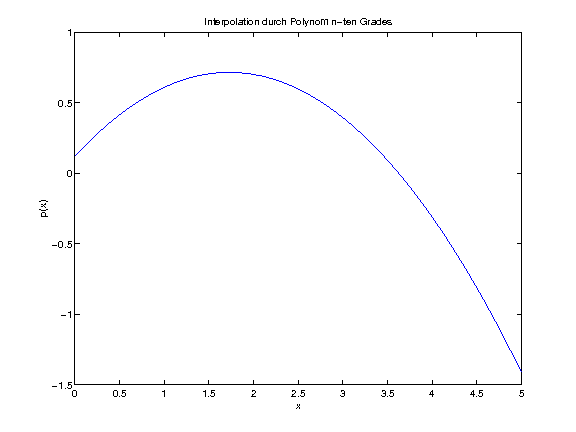
\includegraphics[width=0.3\textwidth]{plot4_2.png} & 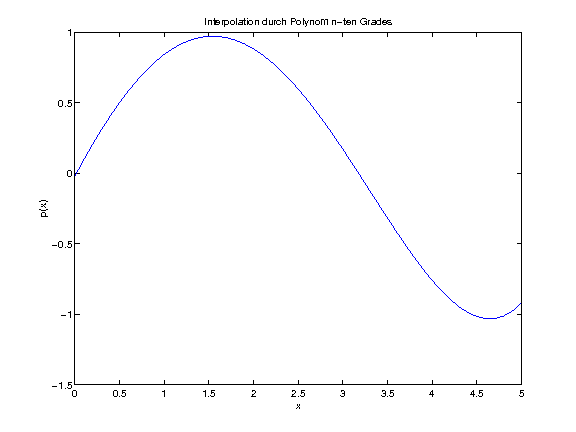
\includegraphics[width=0.3\textwidth]{plot4_4.png} \\
$e^x$ & & & \\
 & 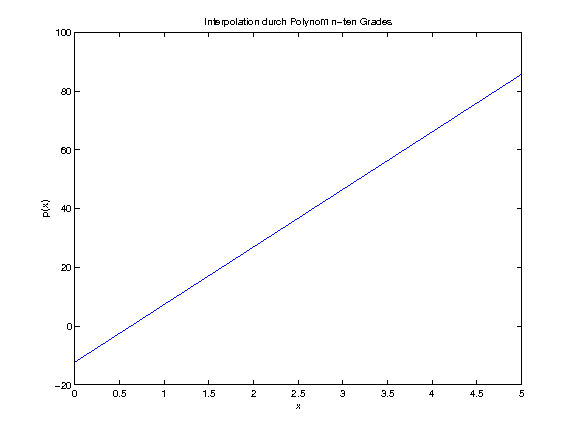
\includegraphics[width=0.3\textwidth]{plot3_1.png} & 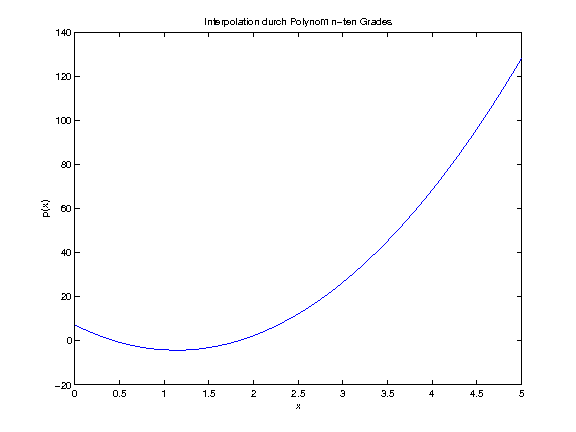
\includegraphics[width=0.3\textwidth]{plot3_2.png} & 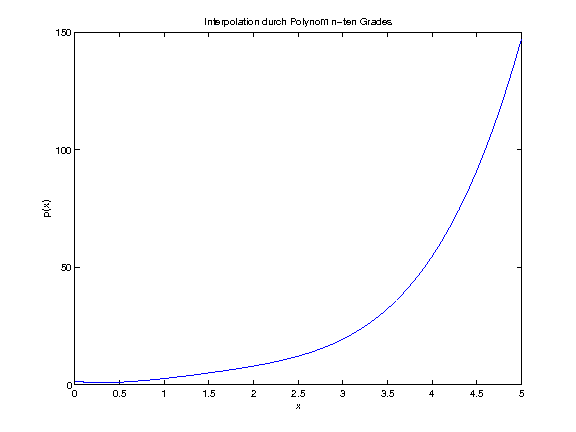
\includegraphics[width=0.3\textwidth]{plot3_4.png} \\
\end{tabular}

\newpage
\subsubsection*{e)}
\textbf{InterpolationAD}: Interpolation mit äquidistantem Gitter ergibt folgende Polynome bzw. Fehlerplots:

\begin{tabular}{l|cc}
n & Interpolationsplot & Fehlerplot \\
\hline
5 & & \\
 & 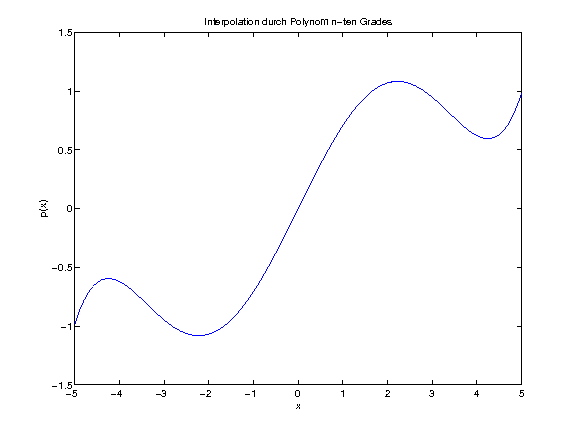
\includegraphics[width=0.45\textwidth]{plotE_AD_5.png} & 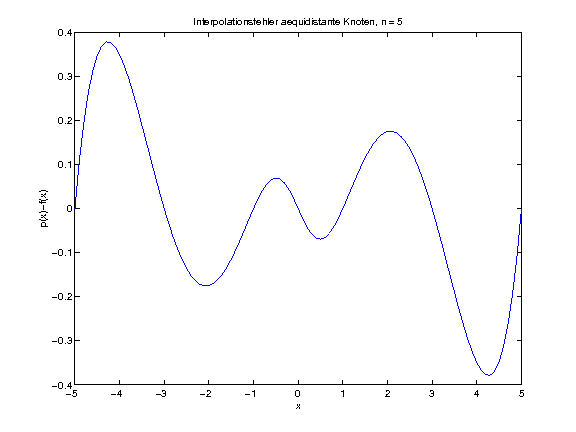
\includegraphics[width=0.45\textwidth]{fehlerAD_5.png} \\ 
25 & & \\
& 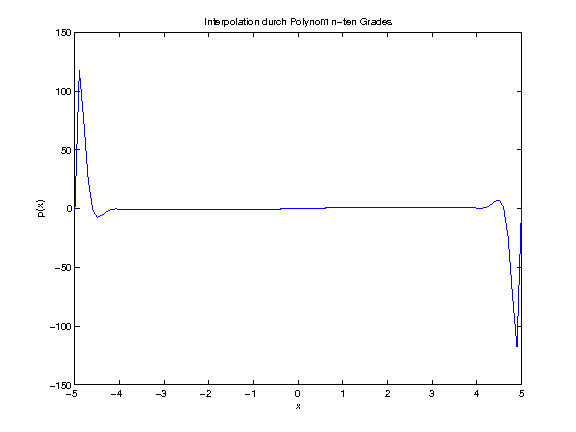
\includegraphics[width=0.45\textwidth]{plotE_AD_25.png} & 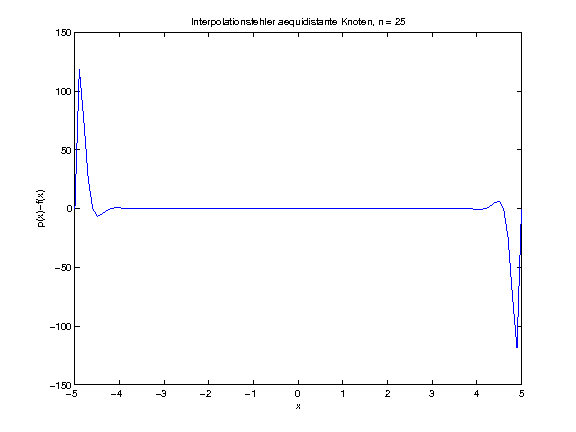
\includegraphics[width=0.45\textwidth]{fehlerAD_25.png} \\
100 & & \\
& 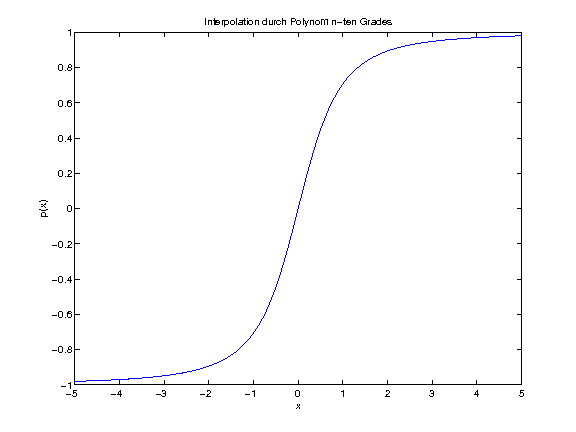
\includegraphics[width=0.45\textwidth]{plotE_AD_100.png} & 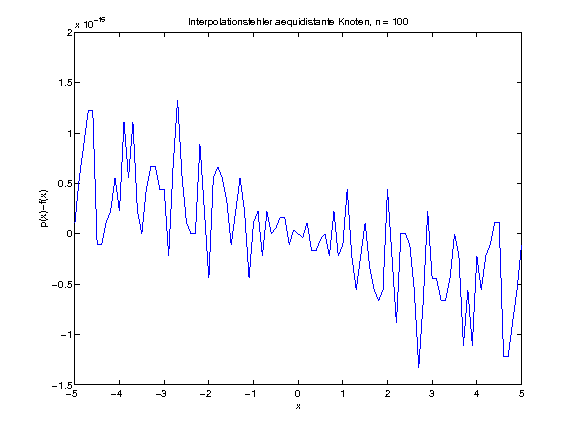
\includegraphics[width=0.45\textwidth]{fehlerAD_100.png} \\
\end{tabular}

\newpage
\textbf{InterpolationTscheby}: Interpolation mit Tschebyschef-Knoten ergibt folgende Polynome bzw. Fehlerplots:

\begin{tabular}{l|cc}
n & Interpolationsplot & Fehlerplot \\
\hline
5 & & \\
 & 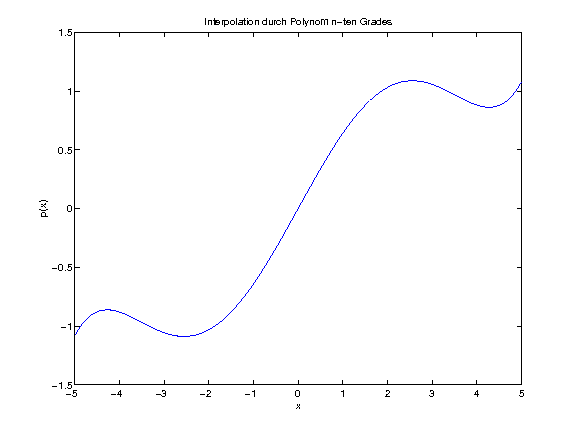
\includegraphics[width=0.45\textwidth]{plotE_TSCHEBY_5.png} & 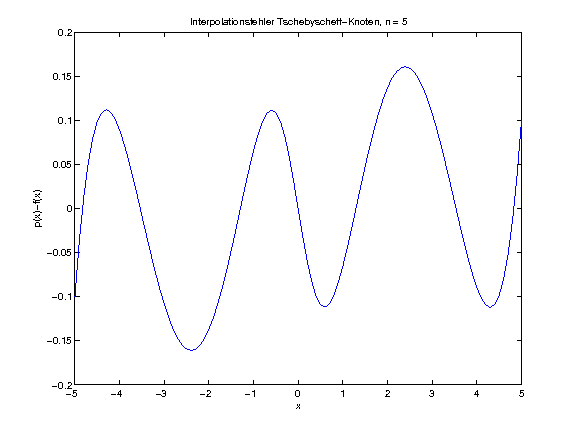
\includegraphics[width=0.45\textwidth]{fehlerTscheby_5.png} \\ 
25 & & \\
& 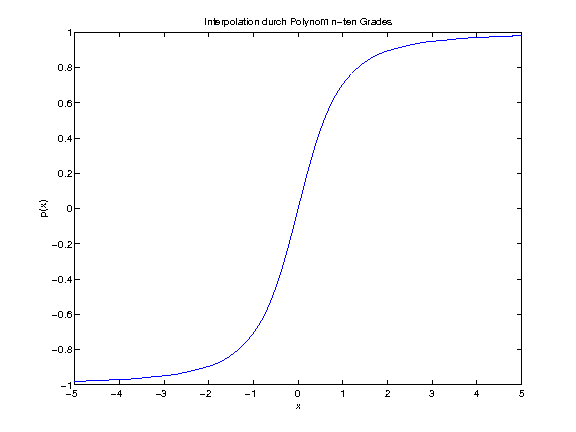
\includegraphics[width=0.45\textwidth]{plotE_TSCHEBY_25.png} & 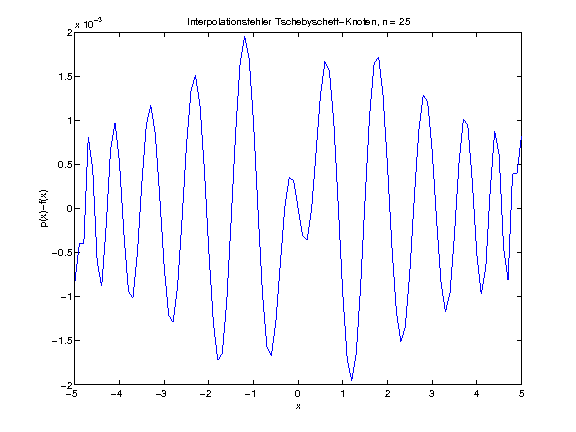
\includegraphics[width=0.45\textwidth]{fehlerTscheby_25.png} \\
100 & & \\
& 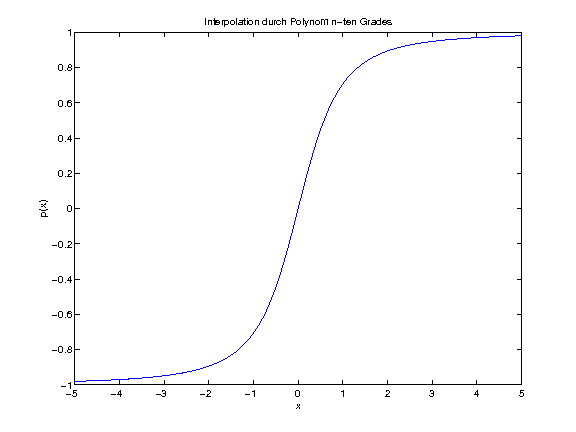
\includegraphics[width=0.45\textwidth]{plotE_TSCHEBY_100.png} & 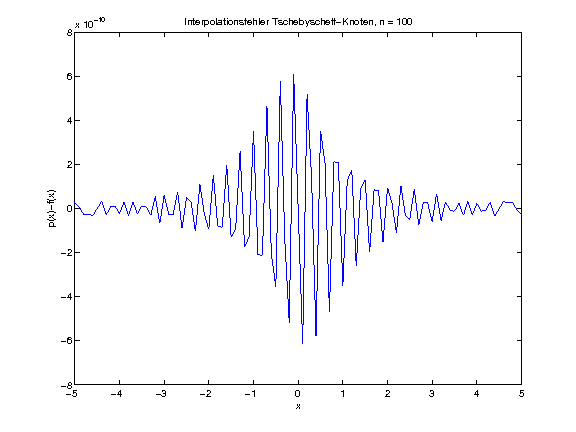
\includegraphics[width=0.45\textwidth]{fehlerTscheby_100.png} \\
\end{tabular}
\label{LastPage}
\end{document}
